\documentclass[a4paper,12pt]{article}
\usepackage{multirow}
\usepackage{graphicx}
\usepackage[utf8]{inputenc}
\usepackage[english]{babel}
\usepackage{hyperref}
\usepackage{longtable,tabu}
\usepackage{pdflscape}
\usepackage{float}
\usepackage{tabularx}
\usepackage{mathtools}
\usepackage{csquotes}
\usepackage[nottoc,numbib]{tocbibind}
\usepackage[backend=biber,style=ieee,sorting=none]{biblatex}
\usepackage{hyperref}
\addbibresource{report.bib}
\hypersetup{
    colorlinks=true,
    linkcolor=blue,
    filecolor=magenta,      
    urlcolor=cyan,
}
\begin{document}


\begin{titlepage}
  \centering
  
\includegraphics[width=0.15\textwidth]{iitkgp.png}\par\vspace{1cm}
  {\scshape\LARGE Indian Institute of Technology, Kharagpur \par}
  \vspace{1cm}
  {\scshape\Large Report \\ for \par}
  \vspace{1.5cm}
  {\huge\bfseries Calculating QoS drop and impact on container during container migration\par}
  \vspace{1.5cm}
  {\large\itshape Mayank Tyagi \textnormal{(16CS60R85)} \\ Abhishek Tiwari \textnormal{(16CS60R83)}\\Sunil Parmar \textnormal{(16CS60R59)}   \\ Rahul Rai \textnormal{(16CS60R35)}\par}
  \vfill
  Supervised by\par
  Dr.~Sandip~\textsc{Chakraborty} \\
  \vfill
  Under The Guidance of\par
  Rohit~\textsc{Dhangar} \\
% Bottom of the page
  \vfill
  {\today\par}
\end{titlepage}




\newpage
\tableofcontents
%\listoffigures
\newpage
\section{Introduction}
\subsection{VM and Docker}
\begin{figure}[H]
  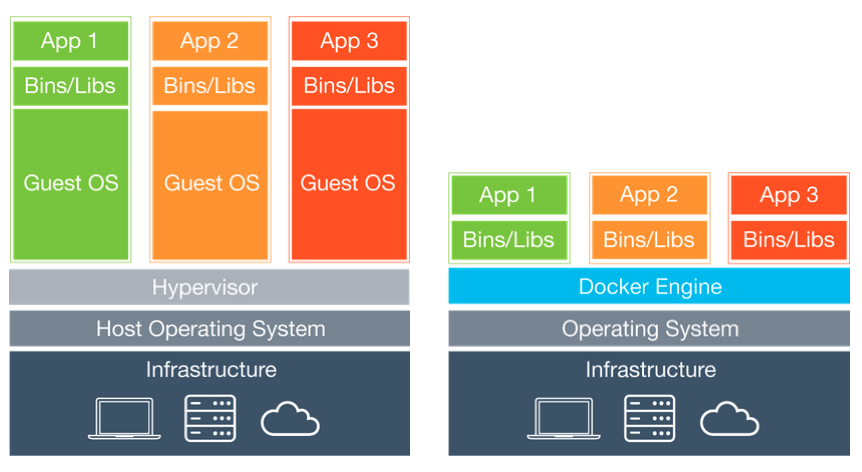
\includegraphics[width=\textwidth]{1.png}
  \caption{VM and Docker}
  \label{fig:fig1}
\end{figure}
\subsubsection{What are virtual machines (VMs) ?}
\begin{enumerate}
\item As server processing power and capacity increased, bare metal applications weren’t able to utilize the new abundance in resources. Thus VMs were born, designed by running software on top of physical servers in order to emulate a particular hardware system.
\item   Hypervisor’s what sits between the OS and hardware and is necessary to virtualize the server.
\item  VMs with different operating systems can be run on the same physical server – a Unix VM can sit alongside a Linux-based VM, etc. 
\item One of the biggest advantage of Server virtualization is the ability to consolidate applications onto a single system.
\end{enumerate}
\subsubsection{What are containers ?}

\begin{enumerate}
\item Operating system (OS) virtualization provides a means to enable software to run predictably and well when moved from one server environment to another. 
\item Containers provide a way to run these isolated systems on a single server/host OS.
\item Each container shares the host OS kernel and, usually, the binaries and libraries, too. Shared components are read-only, with each container able to be written to through a unique mount. 
\item Containers are “shareable” and can be used on a variety of public and private cloud deployments, accelerating dev and test by quickly packaging applications along with their dependencies. Additionally, containers reduce management overhead. 
\item Because they share a common operating system, only a single operating system needs care and feeding (bug fixes, patches, etc).
\item You cannot run a container with a guest operating system that differs from the host OS because of the shared kernel – no Windows containers sitting on a Linux-based host.
\end{enumerate}

\subsubsection{Difference between VM and Container}
VMs and Containers differ on quite a few dimensions, but primarily because containers provide a way to virtualize an OS in order for multiple workloads to run on a single OS instance, whereas with VMs, the hardware is being virtualized to run multiple OS instances. Containers’ speed, agility and portability make them yet another tool to help streamline software development.

\subsection{Ways to migrate containers in docker}
\begin{enumerate}
  \item We can commit the changes in our container to an image with docker commit, move the image onto a new host, and then start a new container with docker run. This will preserve any data that your application has created inside the container.
  \item "Checkpoint and Restore" (CRIU) is an impressive technology demo. Anyways, there was some movement with this in Docker as recently as last year because of how much people want this feature. However, it was decided that there is too much happening in docker-engine to build checkpoint and restore as a feature, and so it was pulled. Now, we know from \#docker on Freenode IRC that checkpoint and restore will be coming back to Docker eventually! Once things settle down in docker-engine.\cite{hvo}
  \item So the applications inside the container needs to be stopped while we move Docker container from one host to another in both the above cases.
\end{enumerate}

\subsection{Downtime}
\begin{enumerate}

\item Since we were unable to find the tool for automated migration of docker containers, measuring downtime with manual migration is ineffcient and is not fit for measuring docker migration downtime. 

\item Since the measure of quality of service depend on downtime, we are unable to compare quality of service measure between VM migrationand docker miration.
\end{enumerate}


\section{Solution/Approach}
\subsection{Testbed Setup}
\subsubsection{How to Setup Container inside docker}
\begin{enumerate}

\item Install packages to allow apt to use a repository over HTTPS: \\
\begin{verbatim} $ sudo apt-get install \ 
  apt-transport-https \
  ca-certificates \
  curl \ 
  software-properties-common
    \end{verbatim}
\item Add Docker’s official GPG key: \\
\begin{verbatim} $ curl -fsSL https://download.docker.com/linux/ubuntu/gpg |
 sudo apt-key add - \end{verbatim}
\item  Use the following command to set up the stable repository.  \\
\begin{verbatim} $ sudo add-apt-repository \ 
   "deb [arch=amd64] https://download.docker.com/linux/ubuntu \ 
   $(lsb\_release -cs) \ 
   stable"
   \end{verbatim}
\end{enumerate}

\subsubsection{Apache Server Setup in Docker Container}
\begin{enumerate}
  \item \textbf{Create Apache Docker container with default settings} \\
  \begin{verbatim}docker run -dit --name apache-web -v "$PWD":/usr/local/apache2/htdocs/
httpd:2.4\end{verbatim}
  \item  \textbf{Enable PHP support in Apache} \\
  To enable PHP support in the Apache webserver, you would have to use an image with Apache and PHP support, say ‘php:7.0-apache’.
\end{enumerate}

\subsection{Tools to migrate container}
\subsubsection{CRIU}
Checkpoint/Restore In Userspace, or CRIU, is a software tool for Linux operating system. Using this tool, you can freeze a running application (or part of it) and checkpoint it as a collection of files on disk. You can then use the files to restore the application and run it exactly as it was during the time of freeze. With this feature, application live migration, snapshots, remote debugging, and many other things are possible.\\
\textbf{Checkpoint :}
There's a top level checkpoint sub-command in Docker, which lets you create a new checkpoint, and list or delete an existing checkpoint. These checkpoints are stored and managed by Docker, unless you specify a custom storage path.
Eg:Creating a checkpoint for a docker image with name looper.\\
\begin{verbatim} $ docker checkpoint create looper checkpoint1 \end{verbatim} 
\textbf{Restore :}
Unlike creating a checkpoint, restoring from a checkpoint just a flag provided to the normal container start call. Here's an example:\\
\begin{verbatim} $ docker start --checkpoint checkpoint1 looper \end{verbatim}

\subsubsection{Flocker}
\begin{enumerate}

\item Flocker is an open-source Container Data Volume Manager for your Dockerized applications. 

\item  By providing tools for data migrations, Flocker gives ops teams the tools they need to run containerized stateful services like databases in production. 

\item  Unlike a Docker data volume which is tied to a single server, a Flocker data volume, called a dataset, is portable and can be used with any container, no matter where that container is running. 
 
\item Flocker manages Docker containers and data volumes together. When you use Flocker to manage your stateful microservice, your volumes will follow your containers when they move between different hosts in your cluster. 

\item You can also use Flocker to manage only your volumes, while continuing to manage your containers however you choose.\cite{dkbbd}
\end{enumerate}

\subsubsection{Kubernetes}
\begin{enumerate}

\item Kubernetes is an open source system for managing containerized applications across multiple hosts, providing basic mechanisms for deployment, maintenance, and scaling of applications. 

\item Kubernetes builds upon a decade and a half of experience at Google running production workloads at scale using a system called Borg, combined with best-of-breed ideas and practices from the community. 

\item Kubernetes is hosted by the Cloud Native Computing Foundation (CNCF). If you are a company that wants to help shape the evolution of technologies that are container-packaged, dynamically-scheduled and microservices-oriented, consider joining the CNCF. For details about who's involved and how Kubernetes plays a role, read the CNCF announcement. \cite{afss}
\item \textbf{Kubernetes Features :}
\begin{enumerate}
\item Automatic Binpacking
  \item Horizontal scaling
  \item Automated rollouts and rollbacks
  \item Service discovery and load balancing
  \item  Secret and configuaration management
  \item Batch Execution
\end{enumerate}

\end{enumerate}

\section{Result}
\begin{enumerate}

\item We were able to do manual migration of containers using above tools but its downtime was dependent on the user migrating the container.
\item We were unable to do a live migration as we do in virtual machine.
\item Manual migration downtime cannot be used to measure Quality of service.
\end{enumerate}


\printbibliography[heading=bibintoc]
\end{document}
